%!TEX root = ../tudkom_students__201804_v1.4.tex
\chapter{Einleitung}
\label{ch:introduction}
% This chapter should motivate the thesis, provide a clear description of the problem to be solved, and describe the major contributions of this thesis.
% 2 pages

\section{Motivation}
% What is the motivation for doing research in this area?
Die Nachfrage nach Wearables steigt kontinuierlich.
Abbildung \ref{fig:stat_wearables} zeigt, dass sich der Absatz in den letzten vier Jahren versechsfacht hat.
Wearables sind Geräte, die am Körper getragen werden, um zum Beispiel mithilfe von Sensoren Daten zu erfassen \cite{definition_wearables}.\\
Ein weit verbreiteter Anwendungsfall ist die Herzfrequenzmessung beim Sport mit einem Fitnessarmband.
Durch das Auswerten dieser Daten kann die Trainingsintensität in Echtzeit an die Person angepasst und somit die Effektivität gesteigert werden.
\begin{figure}[hbtp]
	\centering
	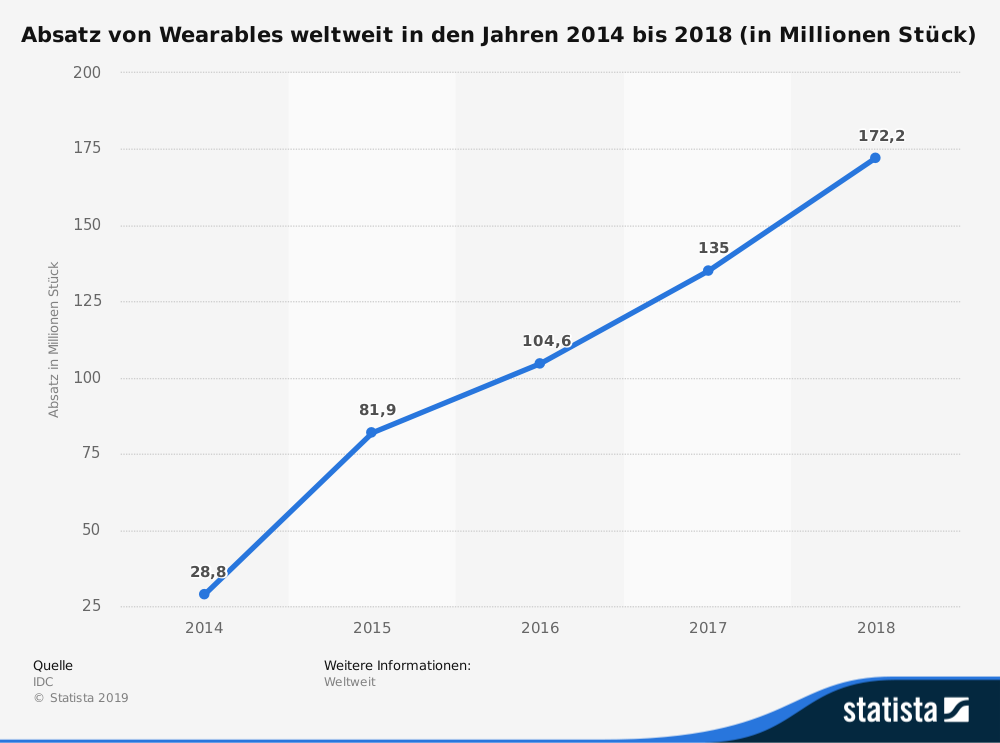
\includegraphics[width=0.75\linewidth]{res/01_statistic_id515723_absatz-von-wearables-weltweit-bis-2018.png}
	\caption{Absatz von Wearables \cite{statistik_wearables}}
	\label{fig:stat_wearables}
\end{figure}\\
In dieser Arbeit hingegen wird ein Wearable entworfen, das die Position und Rotation von Gelenken erfasst.
Auf der Analyse dieser Daten aufbauend können dann weiterführende Anwendungsfälle entwickelt werden.
Folgende sind zum Beispiel interessante Anwendungen:
\begin{itemize}
  \item Das Erkennen von falsch ausgeführten Übungen beim Sport oder falscher Haltung beim Sitzen oder Stehen im Alltag.
	Dadurch können negative gesundheitliche Folgen vermieden werden.
  \item Eine Lösung für mobiles Motion Capturing zum Erstellen von Animationen in Filmen oder Videospielen.
	Mit der Anzahl der Wearables kann die Auflösung der Bewegung proportional zum Preis skaliert werden.
  \item Ein Echtzeitsystem zur Übersetzung von Gestensprache in gesprochene Sprache zur Kommunikation von stummen Menschen.
  \item Für die Bewegungserkennung in Videospielen und Virtual Reality.
	Abbildung \ref{fig:stat_konsolen} zeigt, dass die Nintendo Wii die bisher fünftmeist-verkaufte Konsole ist (Stand: Ende 2018) und damit die Geschichte der Videospielkonsolen prägt.
	Die Fernbedienung übernimmt dabei vor allem eine Funktion: Das Tracken der Handposition.
	Zusätzlich kann man mit dem Nunchuk per Kabel einen zweiten Sensor für die andere Hand anschließen.
	Würde stattdessen eine Konsole mit dem hier entwickelten Wearable entworfen werden, würden die Hände beim Spielen frei bleiben, das Kabel zwischen den Händen wegfallen und es könnten weitere Gliedmaßen getrackt werden.
	VR-Headsets und die Xbox Kinect nutzen dagegen Kameras zur Ganzkörpergestenerkennung.
	Diese Lösung ist dagegen nicht mobil einsetzbar und anfällig auf Störeinflüsse wie fehlender Sichtkontakt.
\end{itemize}
\begin{figure}[hbtp]
  \centering
  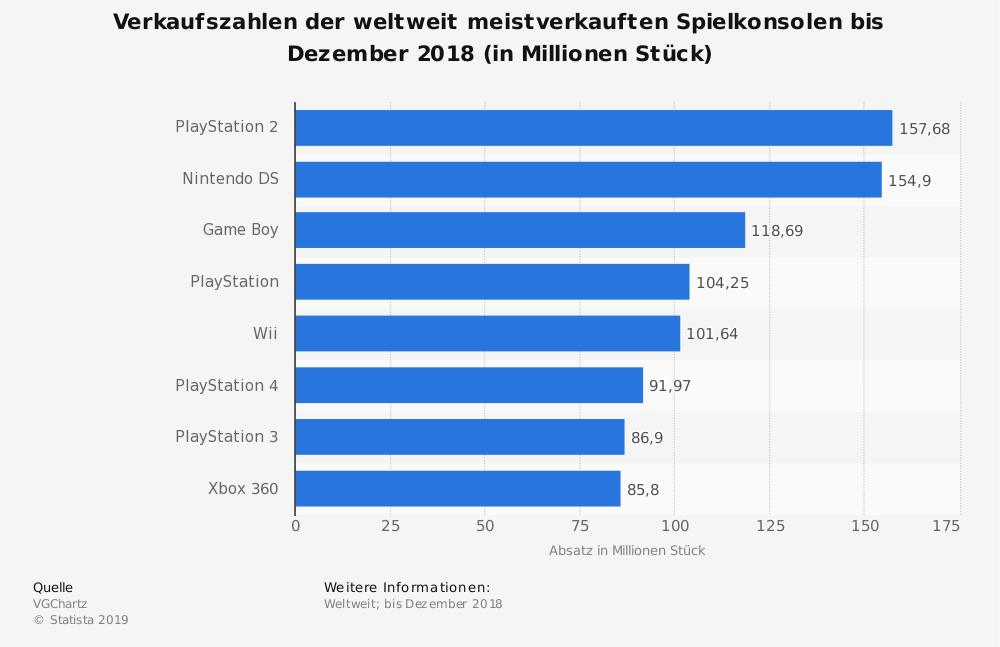
\includegraphics[width=0.75\linewidth]{res/01_statistic_id160549_weltweit-meistverkaufte-spielkonsolen-bis-dezember-2018.png}
  \caption{Verkaufszahlen der weltweit meistverkauften Spielkonsolen \cite{statistik_konsolen}}
  \label{fig:stat_konsolen}
\end{figure}
Das Wearable kann also in vielen Bereichen Anwendung finden. Von Medizin über Kommunikation zur Produktivität und Unterhaltung.

\section{Problemstellung und Beitrag}
% What is the problem that should be solved with this thesis?
\label{ch:aims}
Folgende Ziele ergeben sich für diese Arbeit:
\begin{enumerate}
	\item Um eine gute Mobilität zu gewährleisten, muss das Wearable klein und leicht sein, damit es auch beim Sport praktikabel bleibt.
	\item Die Datenübertragung muss ausreichend schnell sein um die Datenrate zu übertragen, die für Gestenerkennung nötig ist.
	\item Die Energiekapazität und der Energieverbrauch müssen verhältnismäßig zueinander abgestimmt sein.
	Die Batterie soll keinesfalls öfter als einmal pro Tag geladen oder gewechselt werden müssen.
	\item Die eingesetzten Protokolle sollen weit verbreitet sein, damit möglichst viele Endgeräte von dem Wearable profitieren können und bestenfalls einzelne Komponenten des Wearables einfach durch Neuere ersetzt werden können.
\end{enumerate}
Wegen der hohen Mobilität und Verbreitung wurde als Empfänger der Daten ein Smartphone ausgewählt, wobei durch Implementierung der Schnittstelle später auch andere Geräte genutzt werden können.
Das Smartphone soll die Schnittstelle exemplarisch implementieren und die Daten sowie Statistiken zur Verbindung zur Auswertung anzeigen.
Das Wearable soll bei Verbindung Sensordaten mit variabler Rate bereitstellen um Datenübertragung und Energieverbrauch bei verschiedenen Konfigurationen auswerten zu können.

\section{Gliederung}
% How is the rest of this thesis structured?
Zunächst werden verschiedene Protokolle, Techniken oder Komponententypen verglichen, die für das Wearable wichtig sind.
Dann werden bestehende Lösungen vorgestellt und geprüft, welche Vor- und Nachteile sie bieten.
Im Anschluss werden die eingesetzten Komponenten bezeichnet und beschrieben, wie sie miteinander interagieren sollen.
In der Implementierung wird die Beschaltung beschrieben und es werden die Probleme benannt, die bei der Implementierung aufgekommen sind.
Zum Schluss wird das System anhand der genannten Ziele evaluiert und ein Fazit gezogen.
